\section{\Fermi bubbles spectrum}

\subsection{On-off analysis}


\subsection{Low energy data as a background model}

\begin{figure}
	\makebox[\textwidth][c]{
    	\begin{subfigure}{0.3\textwidth}
        	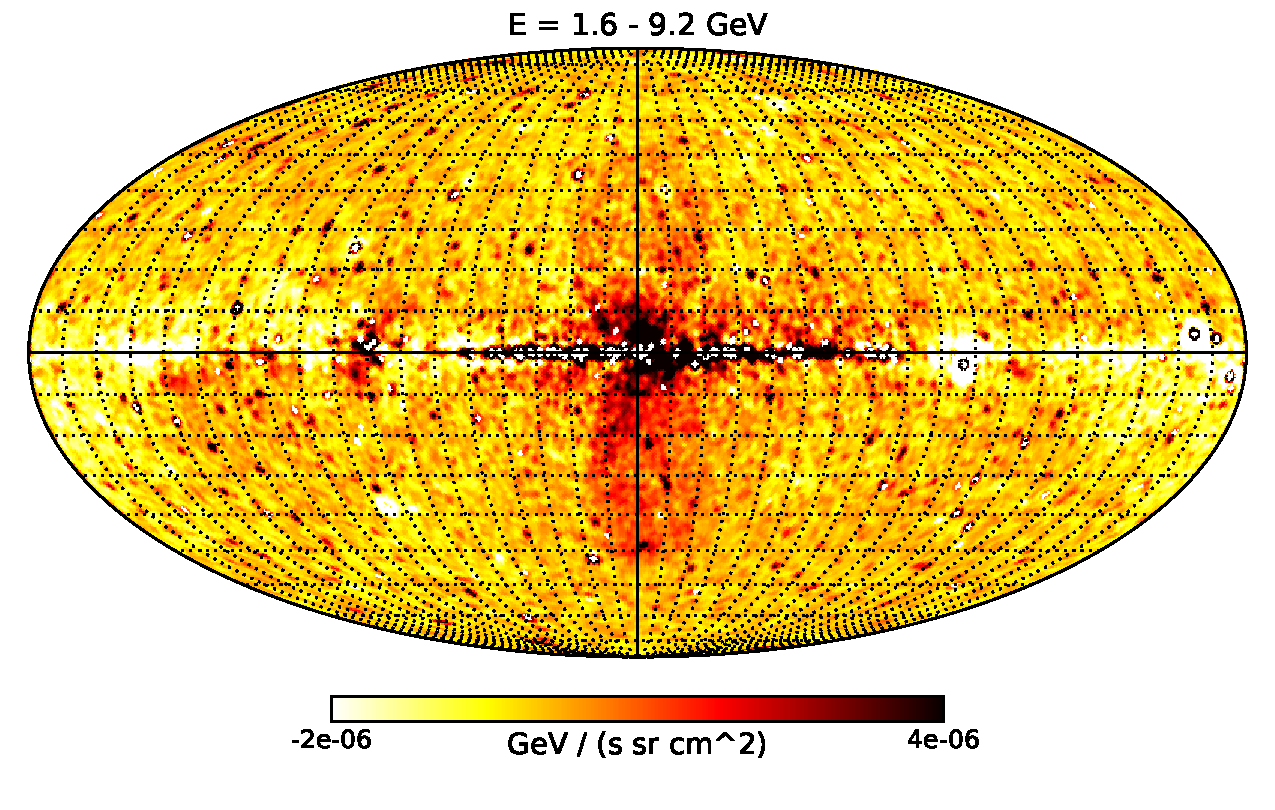
\includegraphics[width=\textwidth]{plots/LowE_06-16GeV_smallmask_bubblesexcl_highEsmooth_symmask_tot_highlow_hot.pdf}
    	\end{subfigure} 
    	\begin{subfigure}{0.3\textwidth}
        	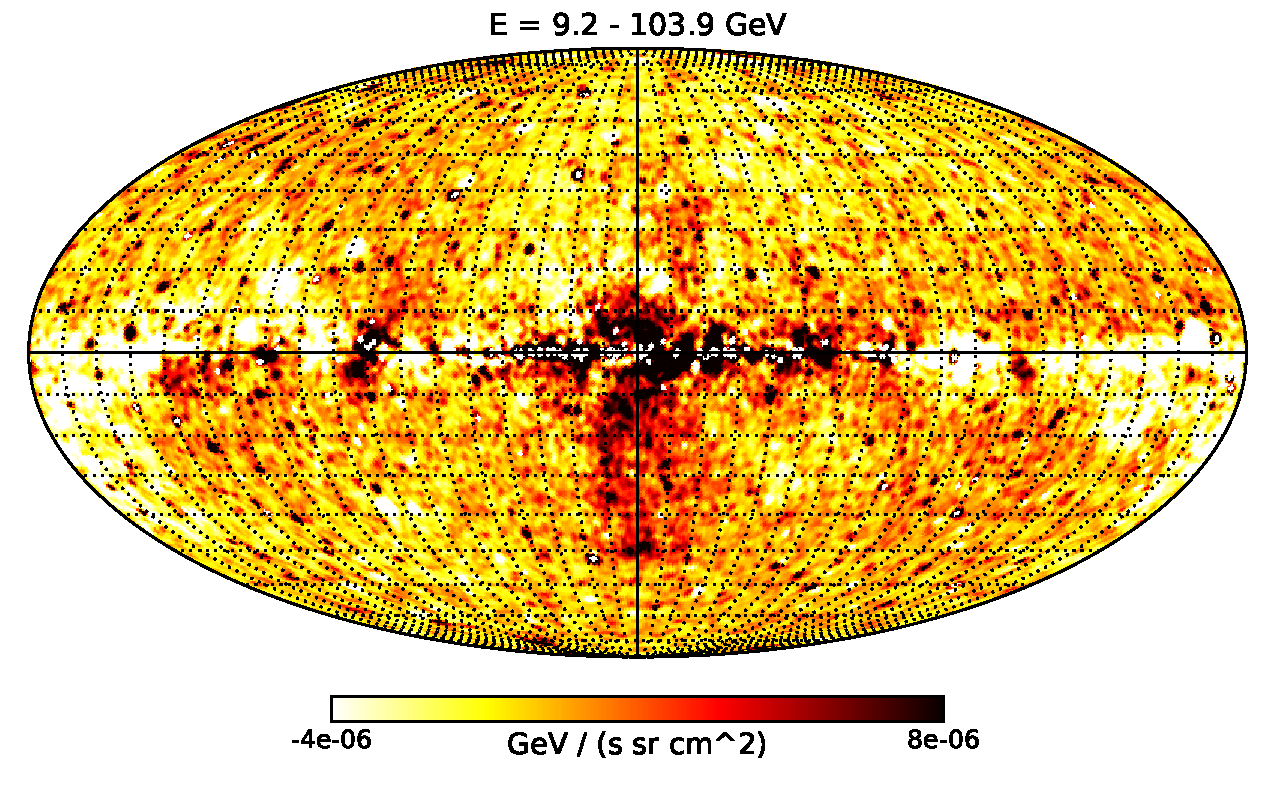
\includegraphics[width=\textwidth]{plots/LowE_06-16GeV_smallmask_bubblesexcl_highEsmooth_symmask_tot_highmedium_hot.pdf}
    	\end{subfigure}
    	\begin{subfigure}{0.3\textwidth}
        	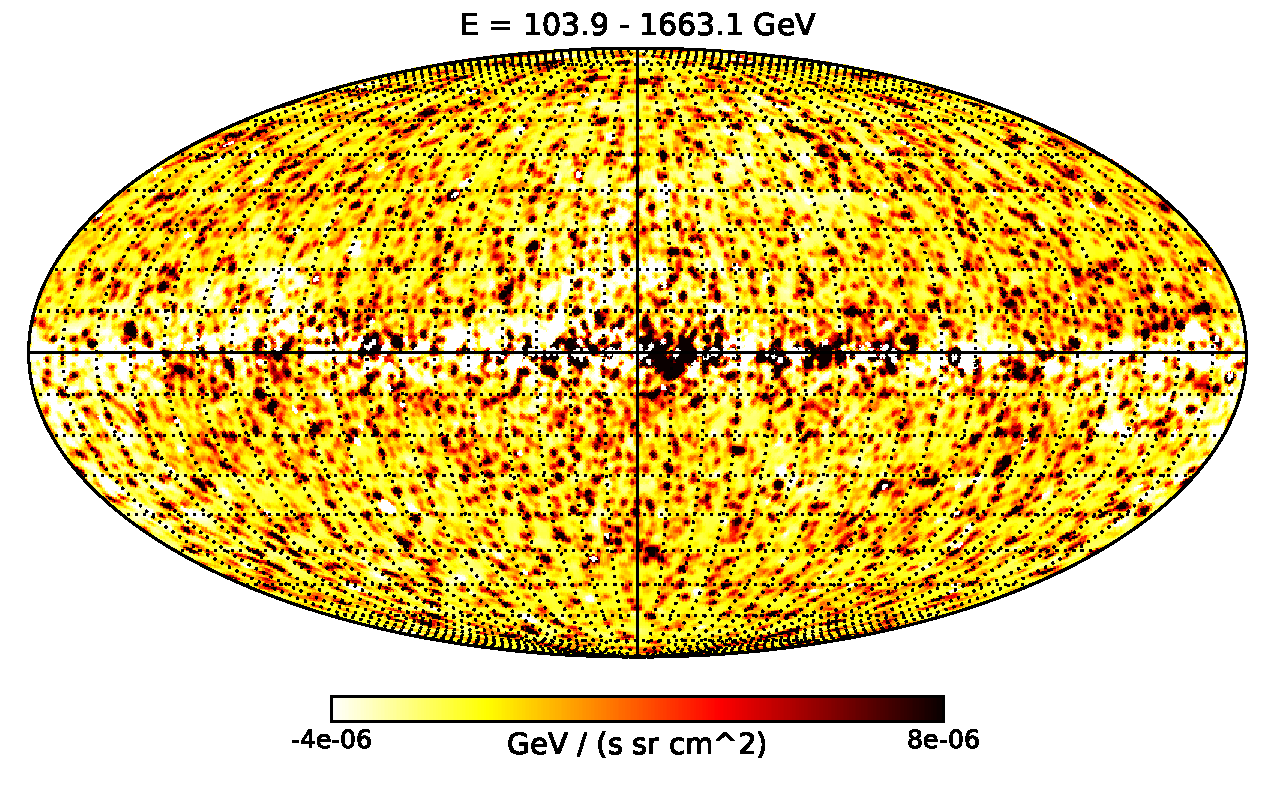
\includegraphics[width=\textwidth]{plots/LowE_06-16GeV_smallmask_bubblesexcl_highEsmooth_symmask_tot_highhigh_hot.pdf}
    	\end{subfigure}
    }
  	\caption{Low-energy model residuals in three different energy ranges.}
\end{figure}


\subsection{Rectangles model of the bubbles}


\subsection{GALPROP model of the foreground and PS refitting}


\begin{figure}
	\makebox[\textwidth][c]{
    	\begin{subfigure}{0.3\textwidth}
        	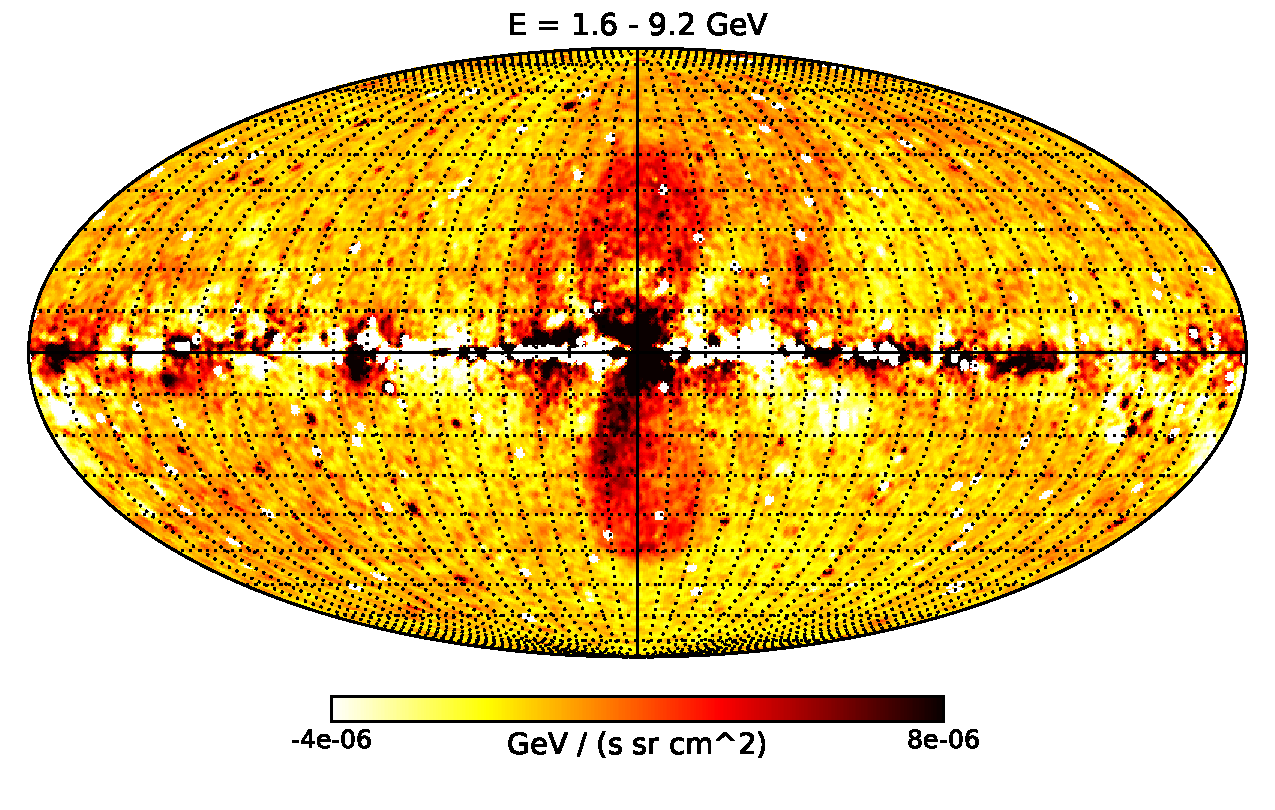
\includegraphics[width=\textwidth]{plots/Source_refit_3FGL_40PS_resid_signal_bubbles_flux_highlowE_hot.pdf}
    	\end{subfigure} 
    	\begin{subfigure}{0.3\textwidth}
        	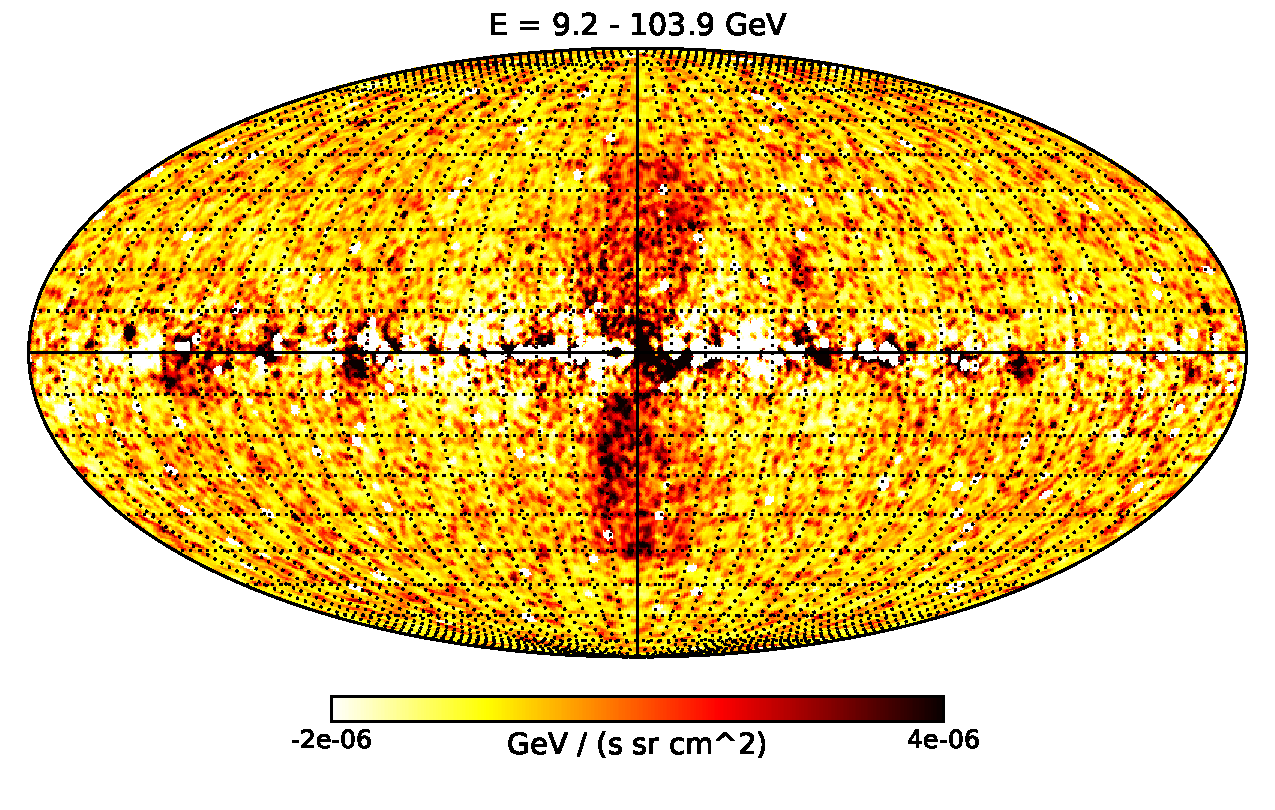
\includegraphics[width=\textwidth]{plots/Source_refit_3FGL_40PS_resid_signal_bubbles_flux_highmediumE_hot.pdf}
    	\end{subfigure}
    	\begin{subfigure}{0.3\textwidth}
        	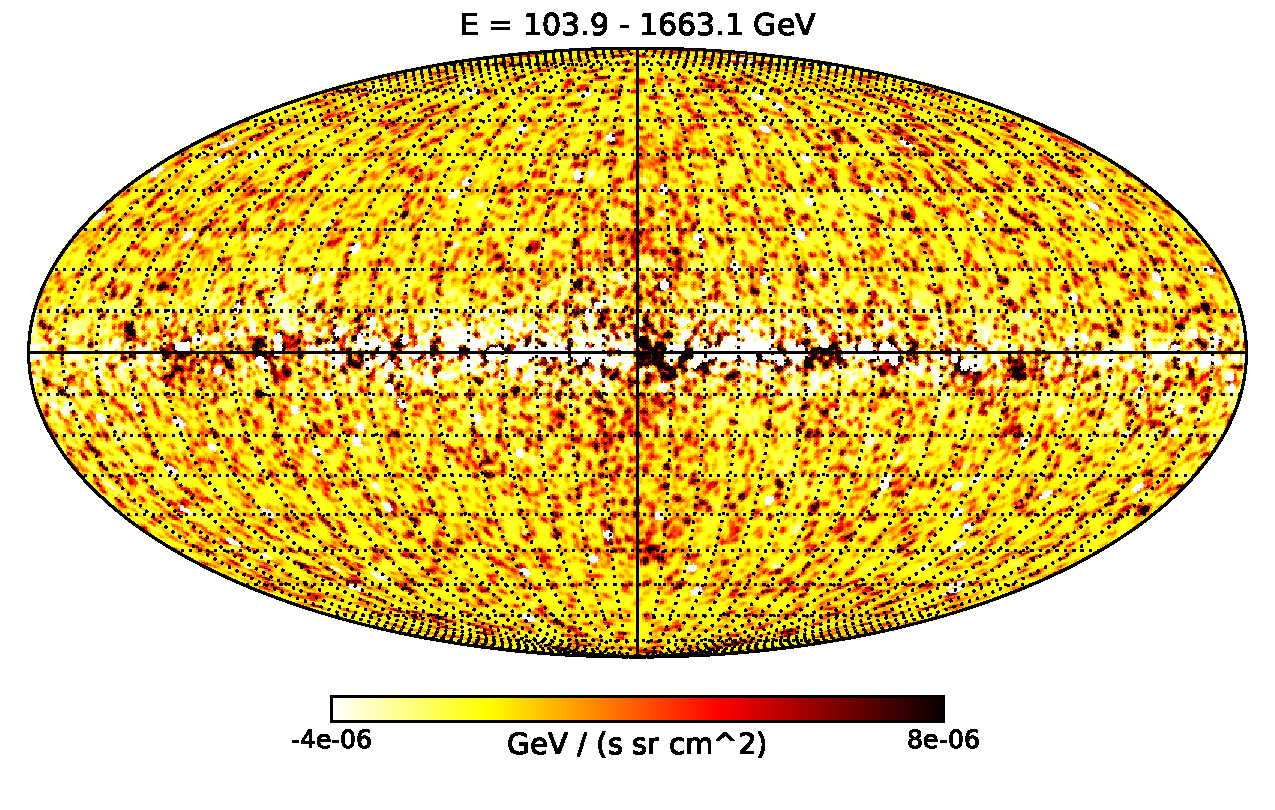
\includegraphics[width=\textwidth]{plots/Source_refit_3FGL_40PS_resid_signal_bubbles_flux_highhighE_hot.pdf}
    	\end{subfigure}
    	}
  	\caption{GALPROP model residuals in three different energy ranges.}
 \end{figure}
